\section{prinsipiell løsning}
\label{sec:concept}

En opamp som vist i figur \ref{fig:02opamp} er en elektronisk forsterker som forsterker differansen mellom to inngangssignalene $v^+$ og $v^-$. Utgangs spenningen $v_o$ vil dermed være lik formel \ref{eq:simplifiedv^o} der $A$ er forstterkningsfaktoren til opampen dette blir også oppgitt i vevsiden \cite{wikipediacontributors_2021_differential}. 

\begin{figure}[H]
	\centering
	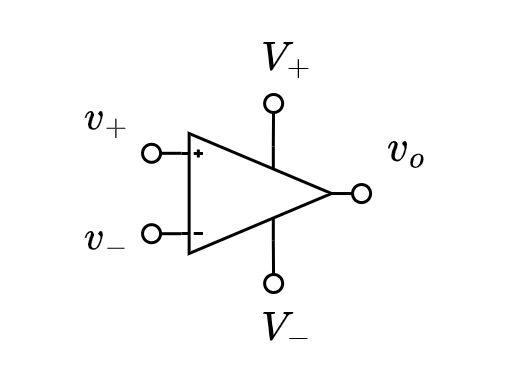
\includegraphics[width=.4\linewidth]{./Images/02Concept/opamp.png}
	\caption{opamp.\cite{pham_2022_selvlaget}}
	\label{fig:02opamp}
\end{figure}

\begin{equation}
    v_0 = A(v^+ - v^-)
    \label{eq:simplifiedv^o}
\end{equation}

$V^+$ og $V^-$ er i dette tilfelle spenningsforsyningen, dette setter også begrensningen for opampen da utgangssignalet $v_o$ vil alltid være $V^- < v_o < V^+$.

I seksjon \ref{sec:issue} er det oppgitt at en idell opamp har en uendelig stor inngangsmotstand og en utgangsmotstand tilnermet 0. Dette gjør at opampen ikke skal påvirke delsytemer som den er koblet til. 

En idé til en slik krets kan være en differentialforsterker som vist i figur \ref{fig:differentialforsterker}

\begin{figure}[H]
	\centering
	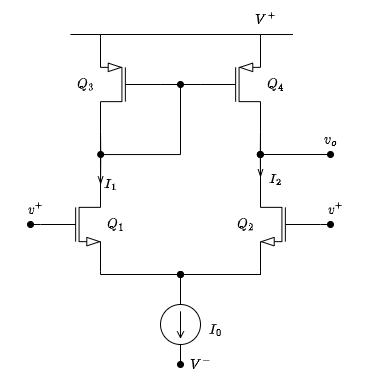
\includegraphics[width=.4\linewidth]{./Images/02Concept/differentialforsterker.png}
	\caption{Differentialforsterker. \cite{pham_2022_selvlaget}}
	\label{fig:differentialforsterker}
\end{figure}




Transistorene $Q_{1}$ og $Q_{2}$ er av typen NMOS mens $Q_{3}$ og $Q_{4}$ er av typen PMOS. På figur \ref{fig:karakteristikkting} tatt fra databladet \cite{stmicroelectronics_2008_2n7000} til en MOSFET transistor er det vist karakteristikken der $I_D$, $V_{GS}$ og $V_{DS}$ er spenningene og strømmene i transistoren i figur \ref{fig:internal}. 

\begin{figure}[H]
	\centering
	\begin{subfigure}{.5\textwidth}
		\centering
		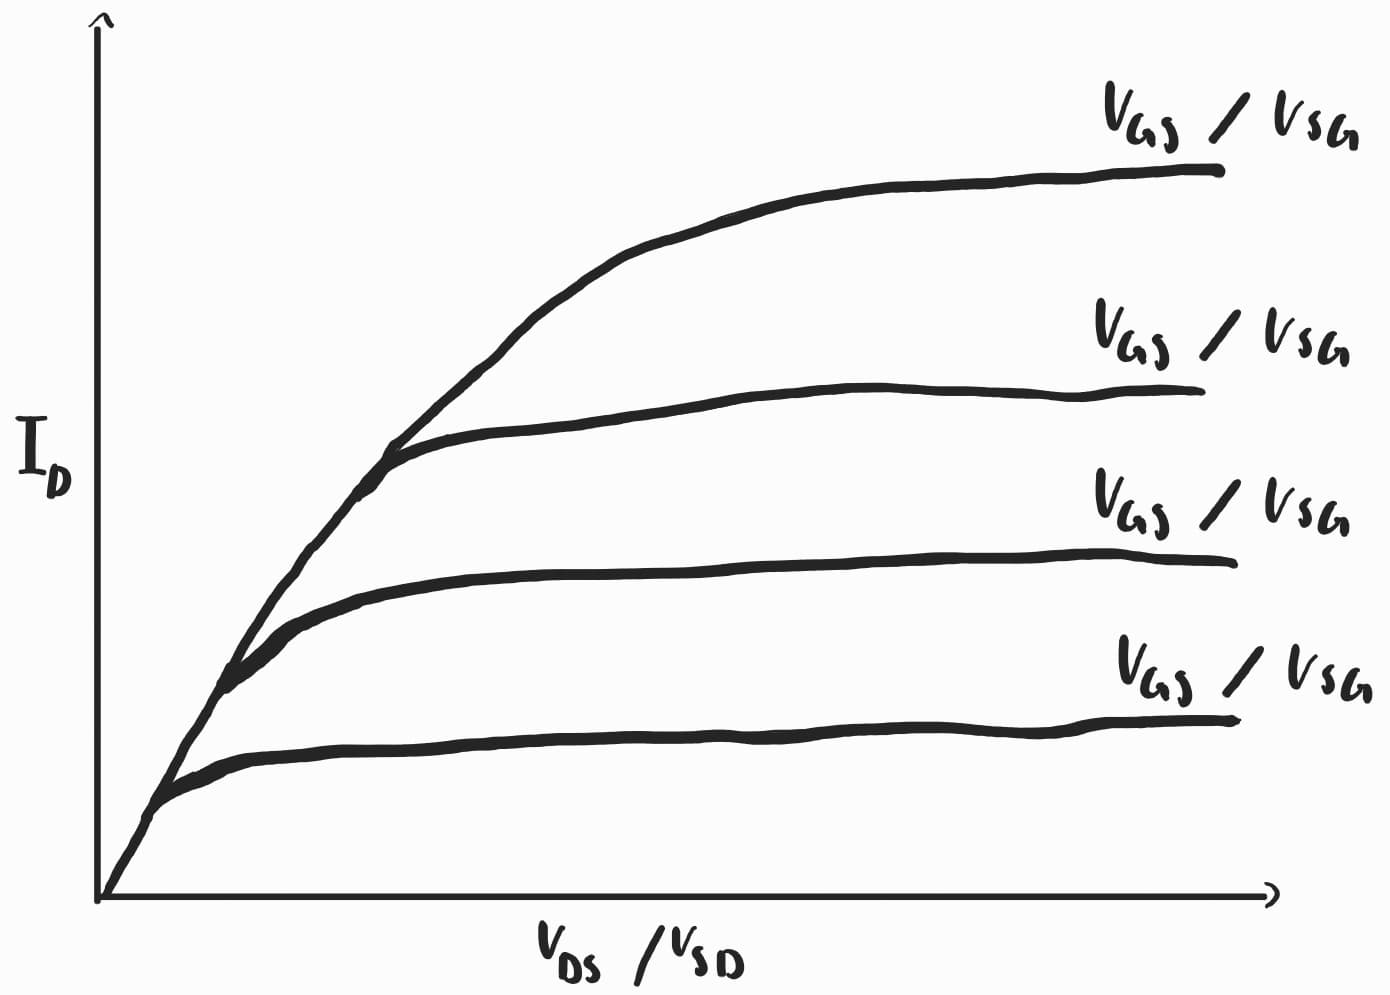
\includegraphics[scale=0.3]{./Images/02Concept/karakteristikkting.jpg}
		\caption{2N7000 NMOS transistor.\cite{stmicroelectronics_2008_2n7000}}
		\label{fig:karakteristikkting}
	\end{subfigure}%
	\begin{subfigure}{.5\textwidth}
		\centering
		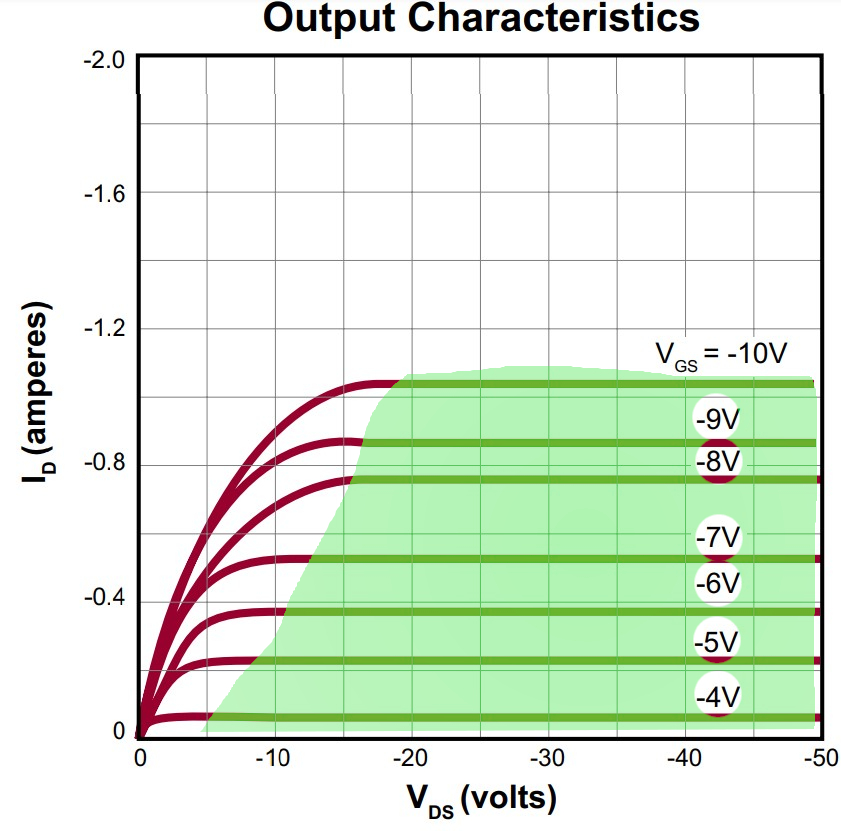
\includegraphics[scale=0.3]{./Images/02Concept/karakteristikkting2.jpg}
		\caption{VP2106 PMOS transistor.\cite{supertex_2013_supertex}}
		\label{fig:karakteristikkting2}
	\end{subfigure}
	\caption{Karakteristikk til MOSFET transistorer}
	\label{fig:karakteristikker}
\end{figure}

\begin{figure}[H]
	\centering
	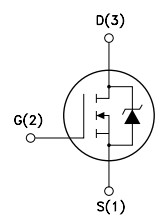
\includegraphics[scale=0.6]{./Images/02Concept/internal.jpg}
	\caption{Intern skjematisk diagram av en 2N7000 MOSFET transistor.\cite{stmicroelectronics_2008_2n7000}}
	\label{fig:internal}
\end{figure}

Fra video \cite{feyling_2022_aktiv} opplyses det at dersom en setter transistorene $Q_3$ og $Q_4$ til å operere i det aktive området, altså det grønne området på figur \ref{fig:karakteristikkting2} hvor det er mest lineært, så vil de ha en liten storsignalmotstand $R$ og samtidig en stor småsignalmotstand $r$. Storsignalmotstand er i dette tilfellet forholdet mellom spenningen $V(I_o)=V_{DS}$ og strømmen $I_o=I_D$ i operasjonspunktet.

\begin{equation}
	R=\frac{V(I_o)}{I_o}
\end{equation}

Mens småsignalmotstanden er er gitt ved forholdet mellom den deriverte av spenningen $dV(I)=dV_{DS}$ og strømmen $I_o=I_D$.

\begin{equation}
	r=\frac{dV(I)}{I}, I=I_o
\end{equation}

Dermed kan man sette spenningen på $V_{GS}$ i forhold til $V_{DS}$ slik at man får ønsket karakteristikk. Som at et lite småsignal på $V_G$ fører til stor $\Delta V_{GS}$, men samtidig så kan det få en relativt stor strøm $I_D$ uten at $\Delta V_{GS}$ er stor.


For å kunne holde $Q_3$ og $Q_4$ i det akrive området uten å måtte manuelt justere på $V_{G}$ blir det forklart i video \cite{feyling_2022_aktiv} at man kan koble gatene til noden mellom $Q_1$ og $Q_3$ som vist i figur \ref{fig:differentialforsterker}. Dette fører dermed til en negativ tilbakekobling som gjør at spenningsnivået til gatene til $Q_3$ og $Q_4$ alltid vil justere seg til riktig nivå.

For å oppnå en lav utgangsmotstand skriver en  av administratorene i vevsiden \cite{admin_2021_mosfet} at kan man legge til en source-følger av typen vist i figur \ref{fig:source} på utgangssignalet. 

\begin{figure}[H]
	\centering
	\includegraphics[scale=0.5]{./Images/02Concept/source_følger.drawio.png}
	\caption{Source følger.\cite{pham_2022_selvlaget}}
	\label{fig:source}
\end{figure}

Strømkilden fra figur \ref{fig:differentialforsterker} kan lages som vist i figur \ref{fig:strømkilde}

\begin{figure}[H]
	\centering
	\includegraphics[scale=0.5]{./Images/02Concept/strømkilde.png}
	\caption{Strømkilde.\cite{pham_2022_selvlaget}}
	\label{fig:strømkilde}
\end{figure}

Her brukes potensiometeret $R_P$ til å justere $V_{GS}$. Dersom man ser på ser på figur \ref{fig:karakteristikkting} kan man se at for lavere $V_{GS}$ spenninger, så vil store endringer i $V_{DS}$ kun føre til små endringer i $I_D$. Dermed så vil man kunne få et veldig stabilt operasjonsstrøm $I_o$.

Hele systemens kretsdiagram er vist i figur \ref{fig:kretsdiagram}.

\begin{figure}[H]
	\centering
	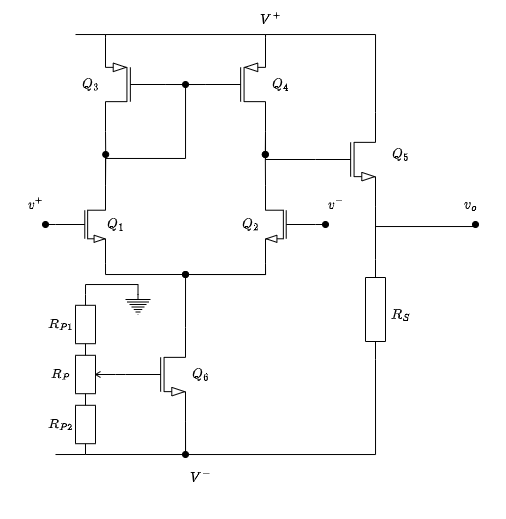
\includegraphics[scale=0.7]{./Images/02Concept/full_kretes.drawio.png}
	\caption{Hele systemets kretsdiagram.\cite{pham_2022_selvlaget}}
	\label{fig:kretsdiagram}
\end{figure}

Her vil spenningsdifferansen $v^+-v^- > 0$ føre til en økt strøm igjennom $Q_1$ og dermed føre til en lavere strøm igjennom $Q_2$ som følge av Kirchhoffs strømlov.
 
 \begin{equation}
	I_o = I_{D_Q1}+I_{D_Q2}
 \end{equation}

 Dette fører igjen til en redussert småsignalmotstand på $Q_4$ som igjen fører til at spenningen $v_o$ blir høyere og motsatt dersom $v^+-v^- < 0$. Med denne kretsen så vil det også gå minimalt strøm mellom inngangenene på transistorene $Q_1$ og $Q_2$, dermed vil man også få en høy inngangsmotstand, som er et av kriteriene.

 Videre så måles Total harmonisk distorsjon (THD) da dette ifølge vevsiden \cite{wikipediacontributors_2022_total} er en måling på den harmoniske distorsjonen i et signal der et lavere distrosjon fører til en mer presis tilnerming til inngangssignalet.

Ved undersøkelse av denne kretsen som en opamp i en ikke-inverterende forsterkerkobling med forsterkning A=10 blir det oppgitt i vevsiden \cite{a2020_glossary} at forholdene mellom motstandene ${R_{I2}} og $${R_{I1}}$ gir en forsterkning lik 

\begin{equation}
    A=1+\frac{R_{I2}}{R_{I1}}
	\label{eq:ikkeinv}
\end{equation}


\begin{figure}[H]
	\centering
	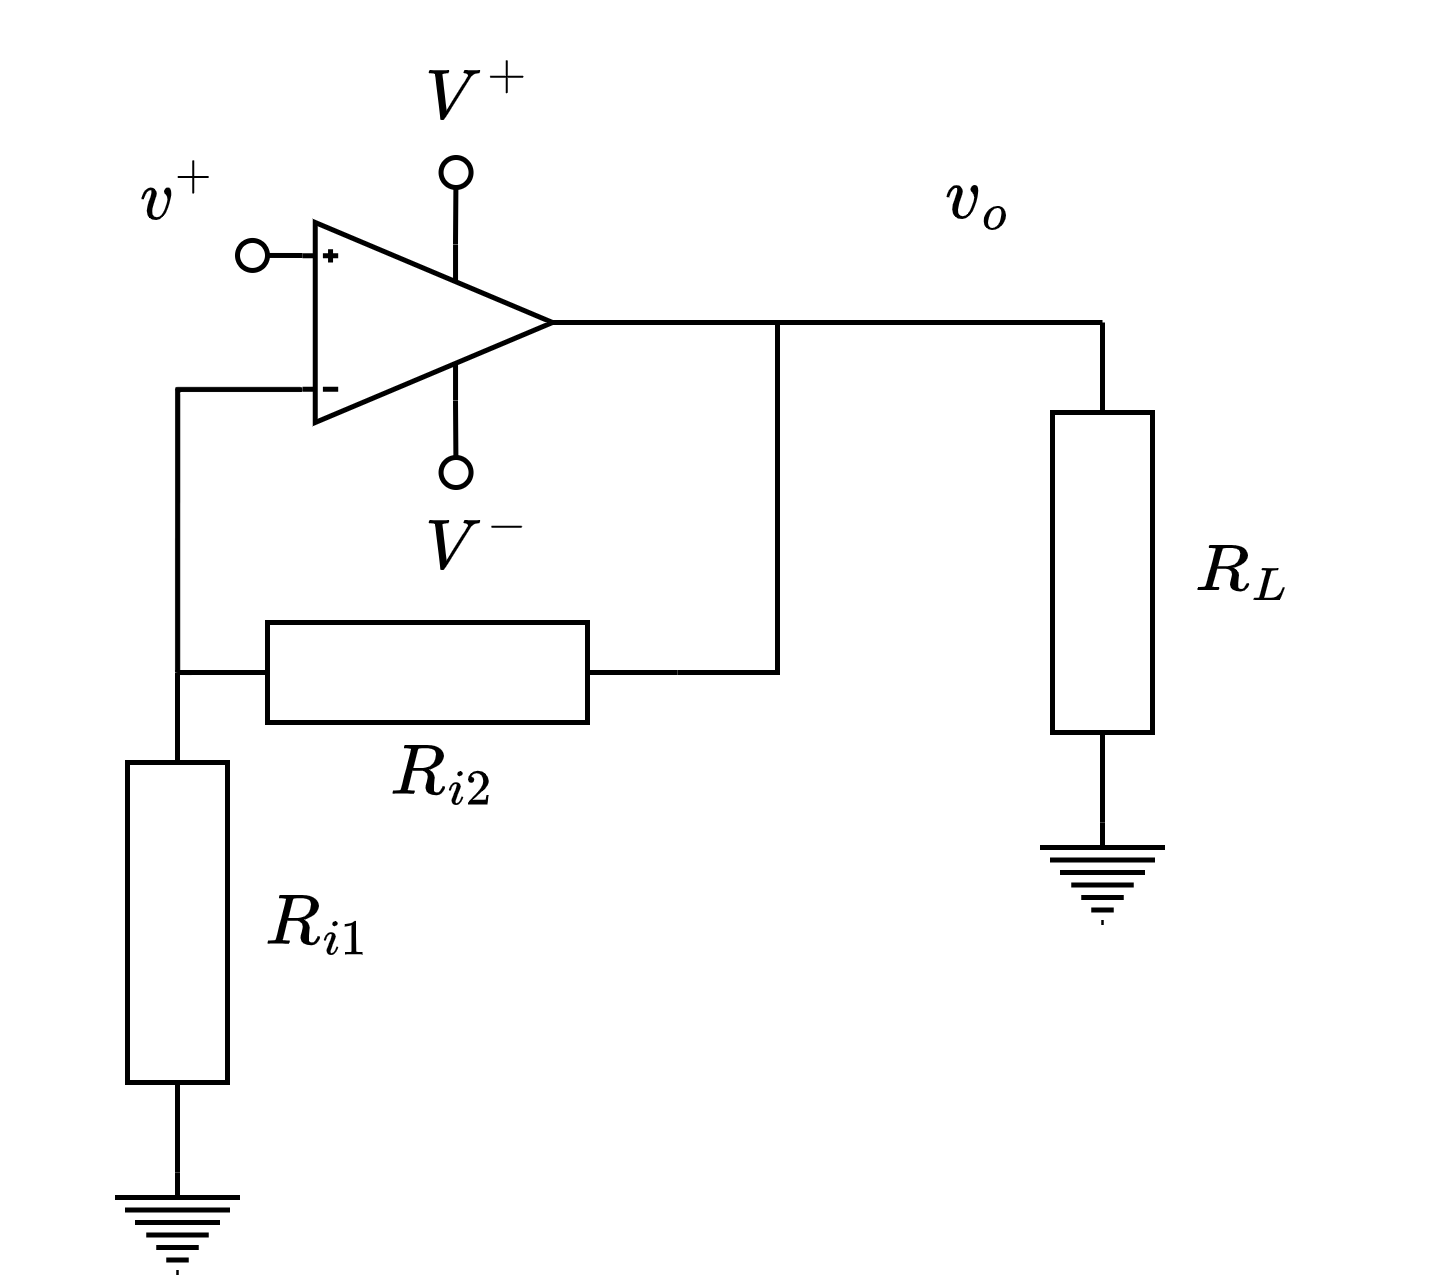
\includegraphics[scale=0.2]{./Images/03Research/ikkeinverterende.png}
	\caption{Ikke-inverterende forsterkerkobling.\cite{pham_2022_selvlaget}}
	\label{fig:Ikke-inverterende}
\end{figure}
